\section{Planned work: Observational measurements}

The new weak lensing tracers we are proposing are unusual in that
observational data already exists which could allow high
significance detections and precise constraints on cosmology. We
therefore plan to move rapidly  to make first detections alongside
our work on mock catalogs,  using those mocks to
inform our estimates of errors and uncertainties.



\begin{figure}[h]
 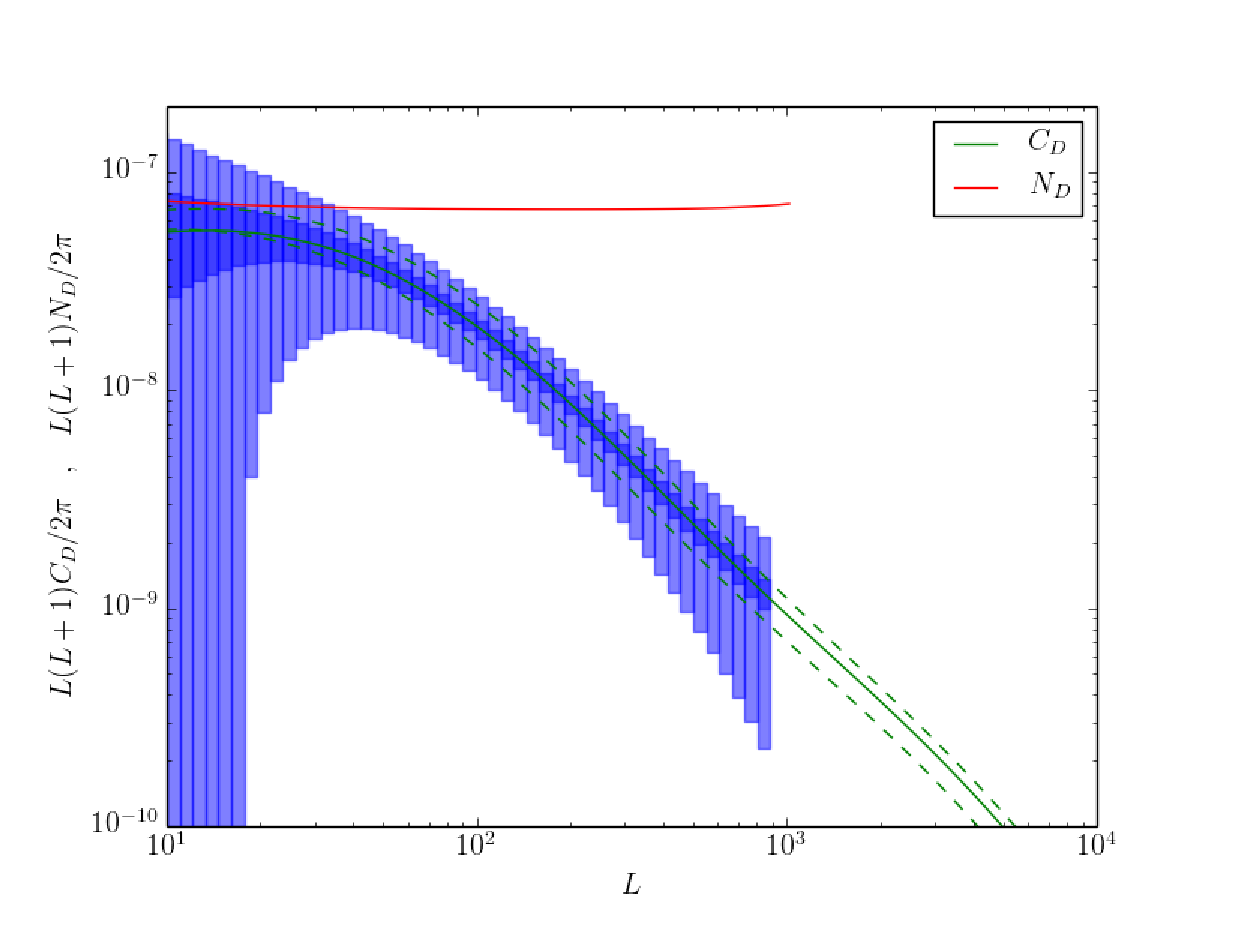
\includegraphics[width=0.5\columnwidth]{figs/eBOSS.eps}
 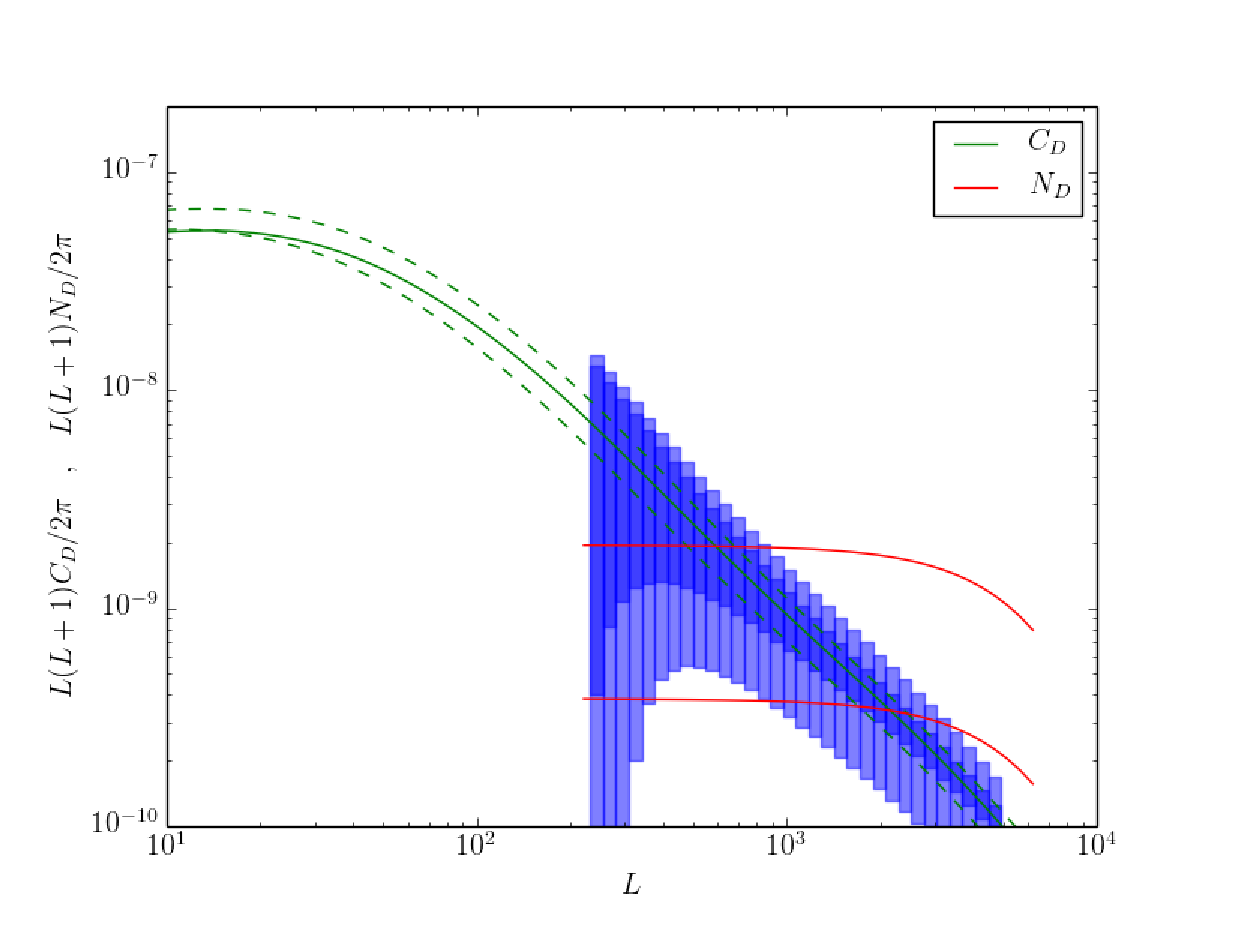
\includegraphics[width=0.5\columnwidth]{figs/CLAMATO.eps}
 \caption{ \footnotesize {\bf The predicted lensing displacement power spectrum  measured
from the \lya\ forest and its 
estimated errors. }
{\bf Left panel:}
eBOSS survey  (see Table~\ref{obs}). The smaller errors are for a redshif
t range $\Delta z =0.5$ and the larger for $\Delta z = 0.1$.  For this survey,  $N_D$ (the noise per 
mode, red line)  is off the range of the plot.  The green curves labelled $C_D$ show the expected power spectra, with the solid curve being for $z_s=2.5$.  For comparison, the upper dashed green curve s
hows results for $z_s=3$ and the lower one for $z_s=2$. {\bf Right panel:}
The CLAMATO survey (\ref{obs}).
The two red curves are the noise in each mode, $N_D$, for the $\Delta z =0.5$ (lower) an
d $\Delta z = 0.1$ (higher) cases.  Where $N_D$ is below $C_D$ high fidelity maps of the lensing convergence is possible.}

 \label{pkpred}
\end{figure}



\begin{table}[h]
\begin{tabular}{|l|l|l|l|l|}
\hline
Dataset   & When      & Area            & N_{\rm spectra} & mean separation \\ \hline
BOSS DR12 & 2016      & 10,000 sq. deg. & 160,000            & 15 arcmin       \\
eBOSS     & 2014-2020 & 7,500 sq. deg.  & 270,000            & 10 arcmin       \\
CLAMATO   & 2014-2020 & 0.8 sq. deg.    & 1,000              & 1.7 arcmin      \\
\hline
\end{tabular}
\centering
\caption{ \footnotesize
{\bf \lya\ forest observational
datasets we will use.} 
Of these, BOSS (Dawson {\it et al.} 2013) has been completed,
eBOSS (Dawson {\it et al.} 2016) and CLAMATO (Lee {\it et al.} 2014, using
galaxy spectra) are ongoing. }
\label{obs}
\end{table}



\subsection{The CLAMATO survey: first detection of \lya\ forest lensing}

The COSMOS Lyman-Alpha Mapping And Tomography Observations (CLAMATO,
\cite{clamato})
 survey is a dense sampling of \lya\ forest spectra in the
COSMOS field, using both quasars and galaxies as backlights.
Some characteristics of the survey are given in Table\ref{obs}. The
sightline density is such that one can expect to make high
fidelity maps of the foreground lensing mass once the survey is completed.
An approximate idea can be gained from Figure \ref{recon} where we show
tests of the reconstruction technique from C18 where the sightline
density was similar to that in the CLAMATO survey. 
CLAMATO has had its first public data release \cite{clamato} and
we will use this data to make what is likely to be the first 
detection of \lya\ forest lensing. A prediction of the 
signal to noise expected in a determination of the lensing mass power spectrum
(taken from the PI's work 
\cite{metcalfandcroft}) is shown in Figure\ref{pkpred}. For
the full survey we expect an 6 \%  constraint on the amplitude
of mass fluctuation $\sigma_{8}$. The first data release contains about
one third of the hoped for final dataset. Galaxy densities are available
to high redshift in the COSMOS field meaning that validation of the
measurement with cross-correlation should be straightforward.

\begin{figure}
  \begin{center}
    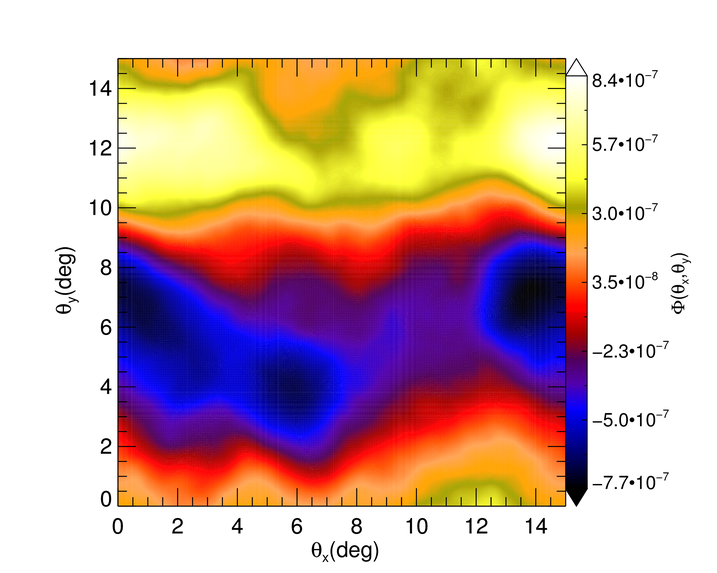
\includegraphics[scale=0.3]{figs/GRP_512_15_z1.png}
    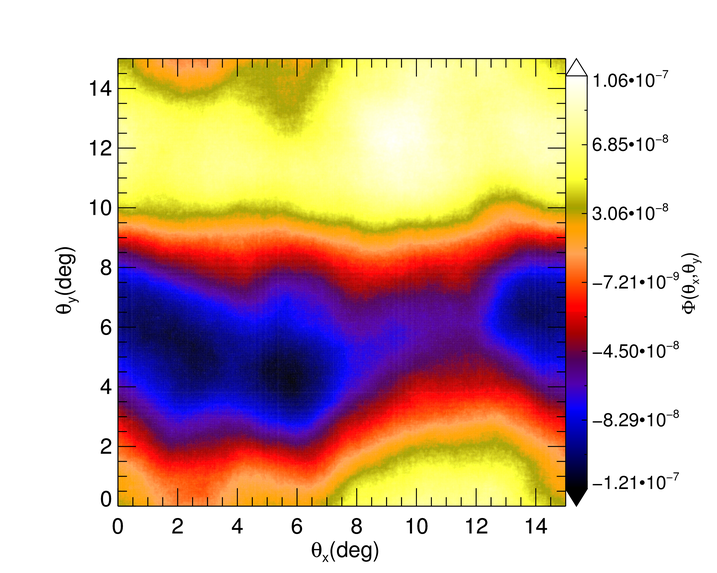
\includegraphics[scale=0.3]{figs/GRP_512_15_z1_Recov.png}
  \end{center}
  \caption{ \footnotesize
{\bf Recovery of the lensing potential field from a simulation of \lya\ forest
lensing}. The left panel shows the input potential and the right panel
the potential reconstructed from a lensed \lya\ forest dataset. The plot is taken from C18, and used gridded forest data (something which will
be improved in our proposed work). The mean spacing of sightlines was 
comparable to that in the CLAMATO survey, which we plan to analyze.
           }
  \label{recon}
\end{figure}

\subsection{eBOSS: 3 percent precision on $\sigma_{8}$}
The eBOSS survey is ongoing, but will be complete early in our project.
It is a large area, low sightline density survey (see Table\ref{obs}), so
that foreground mass maps will have low fidelity. The large area will
however lead to a precise measurement of the power spectrum.
The right panel of Figure \ref{pkpred} shows our prediction from 
\cite{metcalfandcroft}, which yields a 3\% measurement of $\sigma_{8}$.

\subsection{DES clusters: precision stacked cluster mass profiles}

Once tested on simulations, we will apply our
\atf\  method to clusters in the Dark Energy Survey \cite{des2016},
for which the Co-I is co-Chair of the Science Committee. 
As we have shown in Section \ref{sec:lia}, high signal to noise will be
available given that even the year one catalog contains tens of  
thousands of galaxy clusters 
that are selected using the redMaPPer algorithm~\cite{melchior2017}.
Indeed, the amplitude of the stacked cluster profile from year 1 DES data
will have a statistical precision of $1.5 \%$, easily in the 
regime where systematic errors of all methods (such as shear and
lensing magnification) are important, showing that a new method will
be extremely valuable. Along these liness, comparison will 
be made to the shear-based
mass measurements of the same clusters \cite{simet2017} and with
estimates of their mass inferred from the angular clustering
of clusters themselves \cite{baxter2016}.
The estimator codebase developed and used on DES data will
be released to the community so that it can be used, for example, by
all members of the LSST Dark Energy Science Collaboration.
